\section{第一问：感官画像的预测}\label{sec:q1}

第一问要求仅凭 231 个数值输入（226 个化合物与 5 个综合量）预测 50 项感官画像。本文把画像拆成均值、分布和等级三层输出，三层各有对应的损失与评价口径；均分与分布的模型比较在同一套按酒划分的 15 个留出折上完成，区间与缺失实验另设划分，后文分别注明。

\subsection{三类输出与评价指标}

第一问的交付物是三类可分别评价的输出，而不是一个等级。第 3 节已把第 $b$ 款酒、第 $j$ 个属性的面板均分记为 $\bar s_{bj}$，把七级评分分布记为 $q_{bjk}$；本节沿用这两组记号。

交付物包括连续的面板均分 $\bar s_{bj}\in[0,6]$、七维概率 $(q_{bj0},\ldots,q_{bj6})$（非负且和为 1），以及由分布导出的众数等级与中位数等级；前两者描述平均强度与评分分歧，后者给出整数决策。众数取概率最大的等级，中位数取累计概率首次达到 0.5 的等级；在零膨胀的偏态分布下两者经常不同，不能互相替代。

三类输出对应三种决策。若只需要一个总体强度，取面板均分；若要报告不确定性，取七级分布；若必须给出一个整数等级，才在众数和中位数之间选择。把三者压成一个数字，会丢失评分分歧，也会让评价口径随下游任务漂移。

面板均分用平均绝对误差评价：

\begin{equation}
\mathrm{MAE}=\frac{1}{nm}\sum_{b=1}^{n}\sum_{j=1}^{m}\left|\bar s_{bj}-\hat s_{bj}\right|.
\label{eq:mae}
\end{equation}

其中 $n$ 为酒数，$m$ 为核心 30 项或全 50 项，$\hat s_{bj}$ 为留出预测。MAE 的单位是分，可直接与 0—6 的评分尺度对照。

分布质量用累计分布平方距离评价。记某款酒某属性的预测概率为 $\hat p_h$、观测分布为 $q_h$，$P_k=\sum_{h=0}^{k}\hat p_h$ 与 $Q_k=\sum_{h=0}^{k}q_h$ 分别为预测分布与观测面板分布在等级边界 $k$ 的累计概率，则

\begin{equation}
D=\frac{1}{6}\sum_{k=0}^{5}\left(P_k-Q_k\right)^2.
\label{eq:cdd}
\end{equation}

式\eqref{eq:cdd} 对六个内部边界取平均，使 $D$ 与七级概率处于同一尺度；逐条记录计算后取平均，得到表\ref{tab:ordinal} 中的 $D$。$D$ 越小，预测分布越接近该酒实际的面板经验分布。

若把预测分布发给一位随机抽出的品评员，其实际等级为 $Y$，则单次评分的秩序概率评分为

\begin{equation}
\mathrm{RPS}(P,Y)=\frac{1}{6}\sum_{k=0}^{5}\left(P_k-\mathbf{1}\{Y\le k\}\right)^2.
\label{eq:rps}
\end{equation}

式\eqref{eq:rps} 是严格适当的评分规则，鼓励模型报告真实概率而不是把质量压向某一等级\cite{gneiting2007}。对 $Y\sim q$ 取期望，并记面板分歧项 $\Delta=\frac{1}{6}\sum_{k=0}^{5}Q_k(1-Q_k)$，则

\begin{equation}
\mathbb{E}_{Y\sim q}\left[\mathrm{RPS}(P,Y)\right]=D+\Delta.
\label{eq:rpsdecomp}
\end{equation}

式\eqref{eq:rpsdecomp} 说明个人期望 RPS 由两部分组成：第一部分正是 $D$，第二部分 $\Delta$ 只由观测分布的分歧程度决定。核心 30 项上 $D=0.02178$、期望 RPS $=0.11044$，两者相差 $0.08866$，恰好等于面板分歧项的平均值。把 $0.02178$ 称为 RPS，或把 $0.11044$ 当作分布距离，都会把“分布拟合”和“个人评分预测”混为一谈；本文对两者分别报告、分别解释。

从数值看，分歧项 0.08866 远大于 $D$ 的 0.02178，其中分歧项来自面板经验评分分布的离散度；它反映人员及重复评分差异，不能单独识别其成因。这决定了后文的改进重点：继续压低 $D$ 的空间有限，提高个人等级命中率更困难。

\subsection{面板均分预测}

风格中位数是较强的已知风格基线；融合模型与其误差差距较小，需要结合不确定性解释。

面板均分预测以 15 个留出折评价：按风格分层、以酒为单位做三折，重复五次，每款酒在五次中各被留出一次；先把五次留出预测取平均，再按式\eqref{eq:mae} 计算 MAE。这样同一款酒只贡献一个误差，避免重复留出被当作独立样本。

比较的方法包括训练均值、总体中位数、风格中位数、岭回归、极端随机树、梯度提升树，以及极端随机树与梯度提升树的固定等权融合\cite{geurts2006,friedman2001,breiman1996,wolpert1992}。岭回归的正则系数在训练折内选择，其余方法使用预先固定的参数。

三折而非五折，是因为 22 种风格中有 9 种少于 10 款、最少只有 3 款；三折能保证每个训练折仍覆盖全部风格，五次重复则降低单次划分的偶然性。融合权重固定为等权而不是在留出折内学习，是为了避免把模型选择误差带进比较；风格中位数对每个目标只估计一组风格常数，参数个数等于风格数，因而是一个很强的朴素基线。

结果见表\ref{tab:mae}。融合在核心 30 项上的 MAE 为 0.50222 分，在全部 50 项上为 0.43560 分；相对训练均值的降幅分别为 0.10228 分和 0.11319 分。真正需要解释的是这 0.10228 分从哪里来。风格中位数只使用风格标签、不使用任何化合物，核心 MAE 已达 0.50969 分；使用 231 个化学输入的融合模型只把误差压到 0.50222 分，融合低 0.00747 分。

以酒为单位、在固定预测条件下重采样，融合减风格中位数的差值 95\% 区间为 $[-0.01914,0.00418]$，含 0。在本数据与固定预测的重采样口径下，没有足够证据确认融合模型优于风格中位数；这不等于证明化合物信息的条件增量为零。风格中位数到总体均值的误差差，占总体均值到融合模型误差差的 92.7\%，该比例仅为误差对比，不是信息贡献分解。本文报告的区间均为固定预测条件下的重采样区间，未纳入重新训练和模型选择的不确定性。

\subsection{已知风格下的化学输入对照}

为进一步区分风格信息与化学信息，新增相同外层划分和相同极端随机树参数的探索性比较。一个模型只输入风格的独热编码，另一个模型输入同样的风格编码及231个化学字段；两者的预处理均在训练折拟合，并对每款酒的五次留出预测取平均。仍保留按训练折构造的风格中位数作为面向MAE的非树基线。

\begin{table}[t]
\centering\small
\caption{已知风格条件下的面板均分预测对照}\label{tab:styleincrement}
\begin{tabular}{@{}lrr@{}}
\toprule
模型 & 核心30项MAE & 全50项MAE\\
\midrule
风格中位数 & 0.50969 & 0.44712\\
仅风格 ET & 0.51701 & 0.45762\\
风格与化学 ET & 0.50275 & 0.44019\\
\bottomrule
\end{tabular}
\end{table}

核心30项中，风格与化学ET相对于仅风格ET的MAE差为$-0.01426$分，以酒为单位、按风格分层对固定留出预测重采样5000次，95\%区间为$[-0.02427,-0.00395]$；相对于风格中位数的差值为$-0.00694$分，区间为$[-0.01778,0.00398]$。因此，在该固定树模型和已知风格条件下，加入化学字段改善了对仅风格ET的预测，但相对风格中位数的优势尚不确定。两种ET的输入维数不同，\texttt{max\_features}按各自维数取比例，树的候选分裂集合并不完全相同；本对照也不包含重训与模型选择不确定性。

融合相对极端随机树仍有可辨的改进：核心 MAE 低 0.00367 分，融合减 ET 的差值区间 $[-0.00668,-0.00056]$ 不含 0。融合只是把两个已训练好的树模型等权平均，没有引入新信息，模型平均可以降低部分不一致误差；该实验没有将误差变化分解为方差与偏差，故不对来源作唯一归因。

若以平方误差衡量且两模型误差方差相等，记误差相关系数为 $\rho$，等权平均的误差方差为单模型的 $(1+\rho)/2$；$\rho$ 越低，融合收益越大，但平均不会消除系统性偏差。上述推导依赖等方差假设，本实验未验证该假设，不能由MAE差值直接推断方差贡献。

逐目标看，模型差异并不均匀。图\ref{fig:maeheat} 给出 50 项目标在 5 种模型下的 MAE 热图：高误差集中在低方差目标与口感、整体印象类维度，多数目标的模型间色差很小，只有少数目标对模型选择敏感。继续更换回归器最多只能在这些目标上取得局部改进，不能改变整体误差格局。

预测值本身是否可信，还要看校准。把 12500 条留出预测按预测值分成十等份，比较每箱的预测均值与实测均值：十箱中有九箱的偏差不超过 0.04 分，期望校准误差 ECE 为 0.029（图\ref{fig:cal}）。唯一系统偏差在最高一箱，预测 3.19 分、实测 3.31 分，低估 0.12 分。模型在低分段略高估、在高分段压缩，这与树模型对极端值取平均的行为一致。校准良好不等于排序正确：ECE 小说明整体水平没有漂移，非零众数一致率低说明单个等级仍难判对，两者衡量的是不同层面。

\begin{figure}[t]
\centering
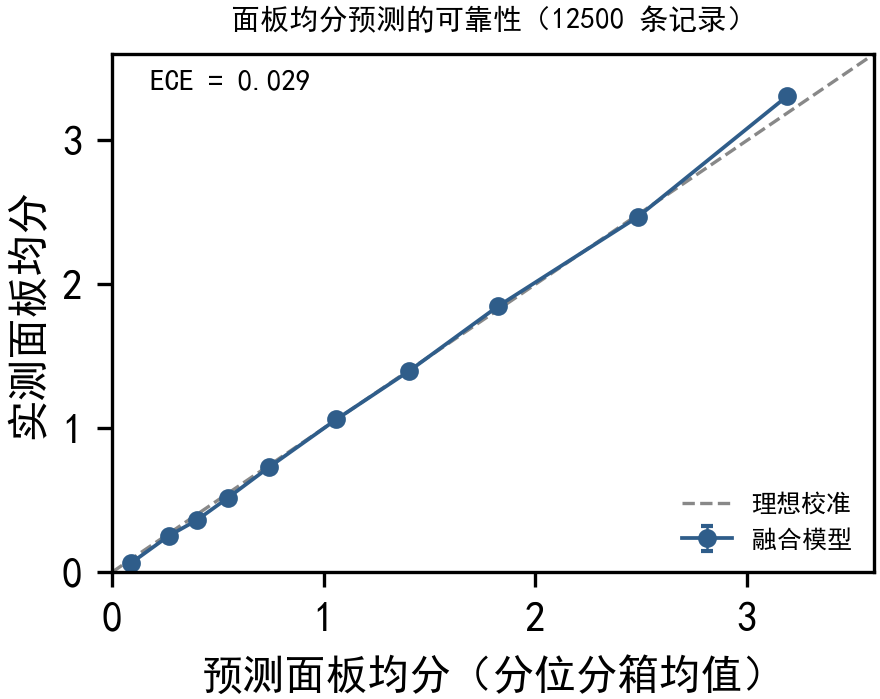
\includegraphics[width=0.92\columnwidth]{figures/fig13_calibration.png}
\caption{面板均分预测的可靠性曲线。十等分箱的实测均值基本落在对角线上，ECE 为 0.029；最高一箱（预测 3.19 分）低估 0.12 分，说明模型压缩了高分端。误差棒为一倍标准误。}
\label{fig:cal}
\end{figure}

逐目标看，最容易的是 \texttt{coriander}（0.108 分）与 \texttt{acetic}（0.166 分），最难的是 \texttt{A\_esters\_isoaa}（0.711 分）、\texttt{A\_esters\_ethac}（0.631 分）与 \texttt{A\_esters\_all}（0.620 分）。难的目标集中在酯类总量与乙酸酯，这类维度在风格间差异大、面板分歧也大，误差不是模型选错造成的。

两个汇总口径也会改变模型排名：核心 30 项上 ET 略好于 GBR（0.50589 对 0.50819），全 50 项上 GBR 反而更好（0.43780 对 0.44336）。单一口径的排名并不稳固，这也是本文同时报告两个口径、并用融合降低单模型波动的原因。

\begin{table}[t]
\centering
\small
\renewcommand{\arraystretch}{1.15}
\caption{七种方法的面板均分留出误差（单位：分）}
\label{tab:mae}
\begin{tabular}{@{}p{0.38\columnwidth}>{\centering\arraybackslash}p{0.27\columnwidth}>{\centering\arraybackslash}p{0.27\columnwidth}@{}}
\toprule
方法 & 核心 30 项/分 & 全 50 项/分 \\
\midrule
训练均值 & 0.60450 & 0.54879 \\
总体中位数 & 0.58785 & 0.52275 \\
风格中位数 & 0.50969 & 0.44712 \\
岭回归 & 0.52270 & 0.45708 \\
极端随机树 & 0.50589 & 0.44336 \\
梯度提升树 & 0.50819 & 0.43780 \\
固定等权融合 & 0.50222 & 0.43560 \\
\bottomrule
\end{tabular}

\vspace{0.3em}
{\footnotesize 注：留出预测为五次留出结果的平均，MAE 以酒为单位计算。}
\end{table}

\begin{figure}[t]
\centering
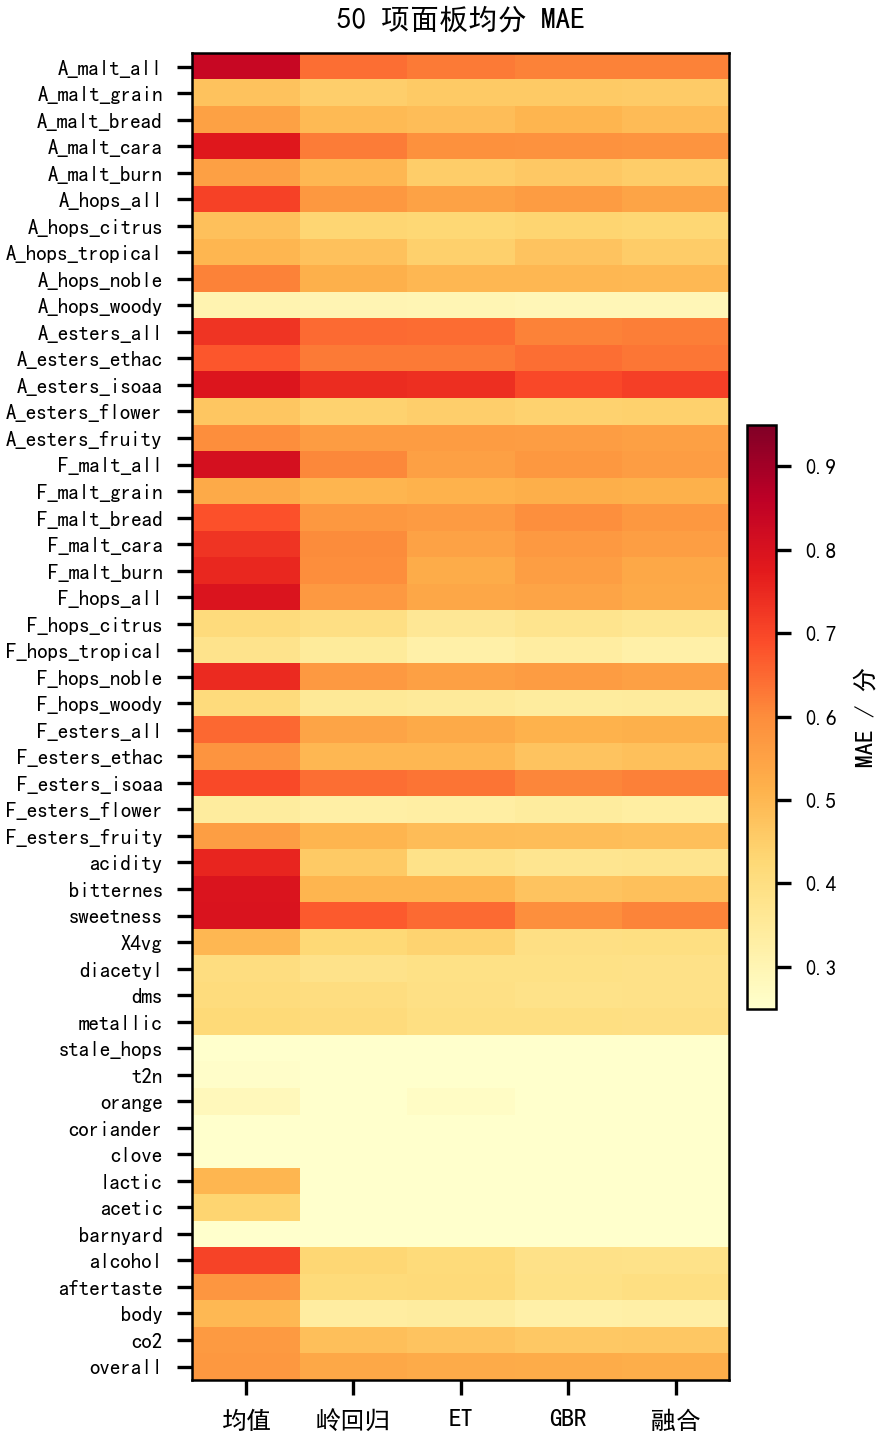
\includegraphics[width=0.95\columnwidth]{figures/fig05_error_heatmap.png}
\caption{50 项目标在 5 种模型下的留出 MAE。误差集中在低方差目标与口感类维度，模型差异只出现在少数目标。}
\label{fig:maeheat}
\end{figure}

\subsection{七级分布与等级识别}

七级分布模型在分布指标上优于两条基线，但总体一致率的提升几乎全部来自零等级；非零等级的识别仍是短板。

以第 3 节的七级分布 $q_{bjk}$ 为监督目标，用多输出极端随机树直接估计七维概率 $\hat p_{bjk}$，再取众数和中位数作为等级输出。表\ref{tab:ordinal} 比较三条路线：训练集的总体经验分布、训练折内的风格经验分布，以及频率极端随机树。三者使用同一套留出折与同一批 7500 条核心记录。

频率 ET 的 $D$ 为 0.02178，低于总体基线的 0.02820 和风格基线的 0.02313；期望 RPS 为 0.11044，低于总体基线的 0.11685 和风格基线的 0.11179。两项分布指标都优于两条基线，化合物信息确实带来改进。

但等级指标给出相反的画面：总体众数一致率 80.52\%，仅比总体基线的 79.31\% 高 1.21 个百分点，还低于风格基线的 80.72\%；非零众数一致率 24.33\%，低于风格基线的 26.58\%。这里出现了指标间的冲突：分布距离和期望 RPS 都支持频率 ET，等级一致率却支持风格基线。冲突的根源是评价对象不同——前两者衡量整条分布，后者只衡量概率最大的那一级；当零等级占近八成时，众数一致率对少数非零等级的错分不敏感。

分布指标改善而等级指标不改善，原因在零膨胀。核心 30 项的 7500 条记录中，观测众数为 0 的占 78.03\%，频率 ET 预测为 0 的占 81.29\%，多出 3.26 个百分点。总体一致率主要由“预测 0 且观测也是 0”撑起；只要把零等级判对，总体一致率就接近 80\%。

零膨胀下的类别不平衡会使总体一致率失真，这是分类评价中的常见现象\cite{hastie2009}。进一步对七个观测等级等权计算宏平均 F1 与平衡准确率，并报告有序等级平均绝对误差。本文保留总体一致率是为了与常规报告口径可比，但同时报告非零一致率，避免用一个被零等级主导的数字下结论。

只看非零记录，识别能力立刻暴露：1648 条观测众数非零的记录中，27.85\% 被预测成 0，只有 24.33\% 的预测等级与观测众数完全一致。属性之间的差异更大：\texttt{A\_hops\_noble} 的 49 条非零记录全部被预测为 0。图\ref{fig:conf} 的混淆矩阵显示，对角线以外的主要误差是把非零等级判为 0，总体一致率掩盖了这部分误差。

针对零膨胀，本文尝试过先判零、再估非零等级的两阶段模型：在与频率模型同为 32 棵树的条件下，非零众数一致率由 24.76\% 升到 25.49\%，提高 0.73 个百分点，但提高幅度的固定条件 95\% 区间 $[-0.91,2.30]$ 个百分点含 0，$D$ 也由 0.02178 升到 0.02200。表中 200 棵树的主模型非零一致率为 24.33\%，与 32 棵树对照的口径不同。证据不足以支持替换，主模型仍取频率 ET；这与 4.2 节的判断一致，化合物输入能修正分布的整体形状，却不足以改变具体等级的排序。

\begin{table}[t]
\centering
\footnotesize
\setlength{\tabcolsep}{1.5pt}
\renewcommand{\arraystretch}{1.15}
\caption{核心 30 项七级分布模型的比较}
\label{tab:ordinal}
\begin{tabular}{@{}p{0.28\columnwidth}>{\centering\arraybackslash}p{0.15\columnwidth}>{\centering\arraybackslash}p{0.15\columnwidth}>{\centering\arraybackslash}p{0.15\columnwidth}>{\centering\arraybackslash}p{0.15\columnwidth}@{}}
\toprule
方法 & $D$ & 期望 RPS & 众数一致率 & 非零一致率 \\
\midrule
总体分布基线 & 0.02820 & 0.11685 & 79.31\% & 21.30\% \\
风格分布基线 & 0.02313 & 0.11179 & 80.72\% & 26.58\% \\
频率 ET & 0.02178 & 0.11044 & 80.52\% & 24.33\% \\
\bottomrule
\end{tabular}

\vspace{0.3em}
{\footnotesize 注：$D$ 与 RPS 无量纲；非零一致率在观测众数非零的 1648 条记录上计算。}
\end{table}

\begin{table*}[t]
\centering\small
\caption{核心30项的留出众数等级补充评价}\label{tab:balanced}
\begin{tabular}{lrrrrr}
\toprule
方法 & 宏平均F1 & 平衡准确率 & 等级MAE & 总体一致率 & 非零一致率\\
\midrule
总体分布基线 & 0.2117 & 0.2490 & 0.4168 & 79.31\% & 21.30\%\\
风格分布基线 & 0.3352 & 0.3184 & 0.4020 & 80.72\% & 26.58\%\\
频率ET & 0.2855 & 0.2835 & 0.3912 & 80.52\% & 24.33\%\\
\bottomrule
\end{tabular}
\par\footnotesize 注：7500个酒—属性记录先合并再按七个实际出现的等级计算宏F1与召回均值；同一酒的30项并非独立观测。风格基线使用已知风格，各折只用训练酒的同风格评分分布。等级MAE按众数等级差计算。
\end{table*}

表\ref{tab:balanced}的平衡准确率和宏F1显示，频率ET低于已知风格基线，而等级MAE较低。三种指标关注的分类与等级距离不同；各方法使用相同外层留出酒和训练折构造基线，风格基线额外依赖风格标签，ET使用化学字段。结果支持保留多种端点及强基线，不支持仅用总体一致率概括非零等级能力。

\begin{figure}[t]
\centering
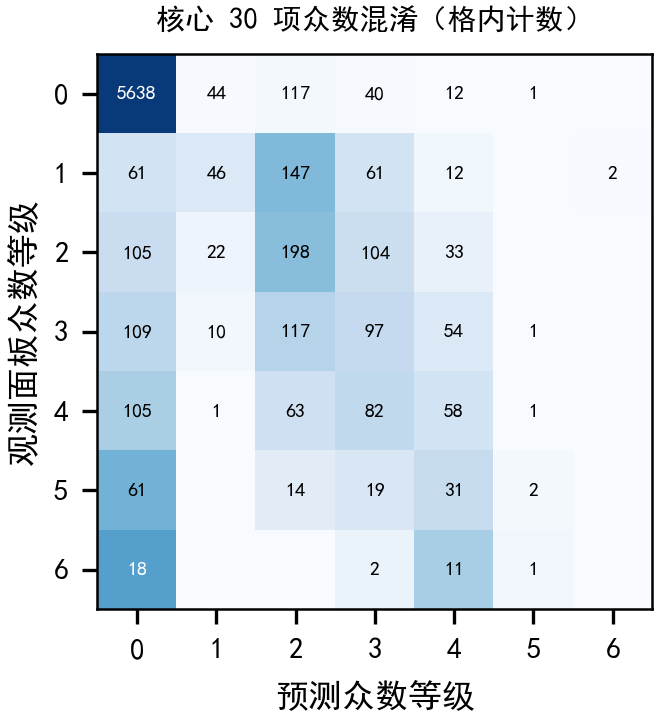
\includegraphics[width=0.95\columnwidth]{figures/fig06_confusion.png}
\caption{核心 30 项留出预测的面板众数等级混淆矩阵。零等级占据对角线的大部分计数，对角线以外的主要误差是把非零等级判为 0。}
\label{fig:conf}
\end{figure}

\subsection{预测区间与缺失条件下的鲁棒性}

保形区间在整体上达到名义覆盖，但在品评人数少的目标上明显不足；缺失机制比缺失比例更能解释性能下降。

区间用五次分割的保形预测构造\cite{lei2018}：每次 150 款酒训练、50 款酒校准、50 款酒测试，按属性在校准集上取绝对残差的分位数，得到该属性的固定半宽。五次分割的逐属性平均覆盖率为 90.06\%，平均宽度为 1.7342 分。覆盖率接近 90\% 的名义水平，说明边际校准是成功的。

保形预测只要求校准集与测试集可交换，不要求残差服从正态分布；按属性分别校准，也避免了跨属性的尺度差异。这两点是它适合面板均分的原因，但也意味着覆盖率是边际的，不是对每款酒、每个人数分组都成立。

边际覆盖不等于条件覆盖。按历史面板人数把测试记录分组，3—4 人组（12 款酒）覆盖率只有 74.00\%，5—7 人组为 86.89\%，8 人及以上组为 92.94\%，随人数单调上升。人少时面板均分本身的抽样噪声更大，而区间半宽按属性统一给出，没有随该酒的实际人数调整，于是小面板目标的残差更容易超出区间。图\ref{fig:cov} 同时给出分组覆盖与面板人数分布：3—4 人组覆盖明显偏低，说明“人少的目标区间不可信”。

分组覆盖的单调性同时给出了使用建议：对 3—4 人的酒样，应把区间宽度按人数放大，或直接标注覆盖不足；对 8 人以上的酒样，现有半宽偏保守，可以适当收窄。区间宽度目前按属性统一估计，尚未利用品评人数这一协变量。

缺失实验分两块。一块在测试阶段叠加完全随机缺失（MCAR），用训练阶段拟合的插补参数填补；15 折聚合下，核心 MAE 由 0.51086 升到 0.52662（20\% 缺失），众数一致率由 80.51\% 降到 80.33\%。这一块只回答随机丢数的代价，不覆盖系统性缺失。

另一块固定 3 折、重复 2 次，使用 300 棵树的 ET，基准 MAE 为 0.50666，分别施加 MCAR（10\%、20\%）、MAR（20\%）、整块通道缺失（20\%）和低值非随机缺失（MNAR，20\%）五个条件，结果见表\ref{tab:missing} 与图\ref{fig:missexp}。

同为 20\% 缺失比例，MNAR 低值条件的 MAE 增量为 $+0.02727$ 分，约为 MCAR 20\%（$+0.01393$）的两倍，也高于 MAR 20\%（$+0.01148$）；整块通道缺失的代价反而最小（$+0.00695$），约为 MCAR 20\% 的一半。缺失机制比缺失比例更重要：随机丢失只是减少信息量，系统性低值缺失还改变了“未检出”与“低浓度”的对应关系，插补会把缺失填向条件均值，模型因而失去区分低浓度样品的能力。同一条件下等级精确率由 0.5399 降到 0.5088，Spearman 相关由 0.4472 降到 0.3985，退化不限于均分。

四类机制的差别可以用缺失与取值的依赖关系解释。MCAR 下缺失与浓度无关，插补误差只来自信息减少；MAR 下缺失可由已观测变量解释，插补还能利用部分信息；整块缺失相当于删掉一个输入通道，剩余通道仍保留大部分信号，在 20\% 比例下代价最小；MNAR 低值缺失直接依赖未观测的低浓度，插补会把低值拉向条件均值，系统性偏差最大。

因此，题面所说的“数据缺失”不能只按缺失比例做压力测试：对仪器数据，低值缺失和整通道未测是两种不同的机制，前者对感官预测的伤害更大。两套缺失实验的基准不同：15 折 MCAR 压力的基准是 0.51086，新增机制实验的基准是 ET-300 的 0.50666，折数与模型设置都不同，两个基准不能直接相减。本文只在各自实验内部比较增量，避免把口径差异误读为机制效应。

\begin{table}[t]
\centering
\small
\renewcommand{\arraystretch}{1.15}
\caption{六种缺失条件下的核心 30 项 MAE 增量（单位：分）}
\label{tab:missing}
\begin{tabular}{@{}p{0.52\columnwidth}>{\centering\arraybackslash}p{0.34\columnwidth}@{}}
\toprule
缺失条件 & MAE 增量/分 \\
\midrule
无缺失 & 0 \\
MCAR 10\% & $+0.00656$ \\
MCAR 20\% & $+0.01393$ \\
MAR 20\% & $+0.01148$ \\
整块通道 20\% & $+0.00695$ \\
MNAR 低值 20\% & $+0.02727$ \\
\bottomrule
\end{tabular}

\vspace{0.3em}
{\footnotesize 注：基准为 ET-300 的 0.50666 分；增量为相对无缺失条件的差值。}
\end{table}

\begin{figure*}[t]
\centering
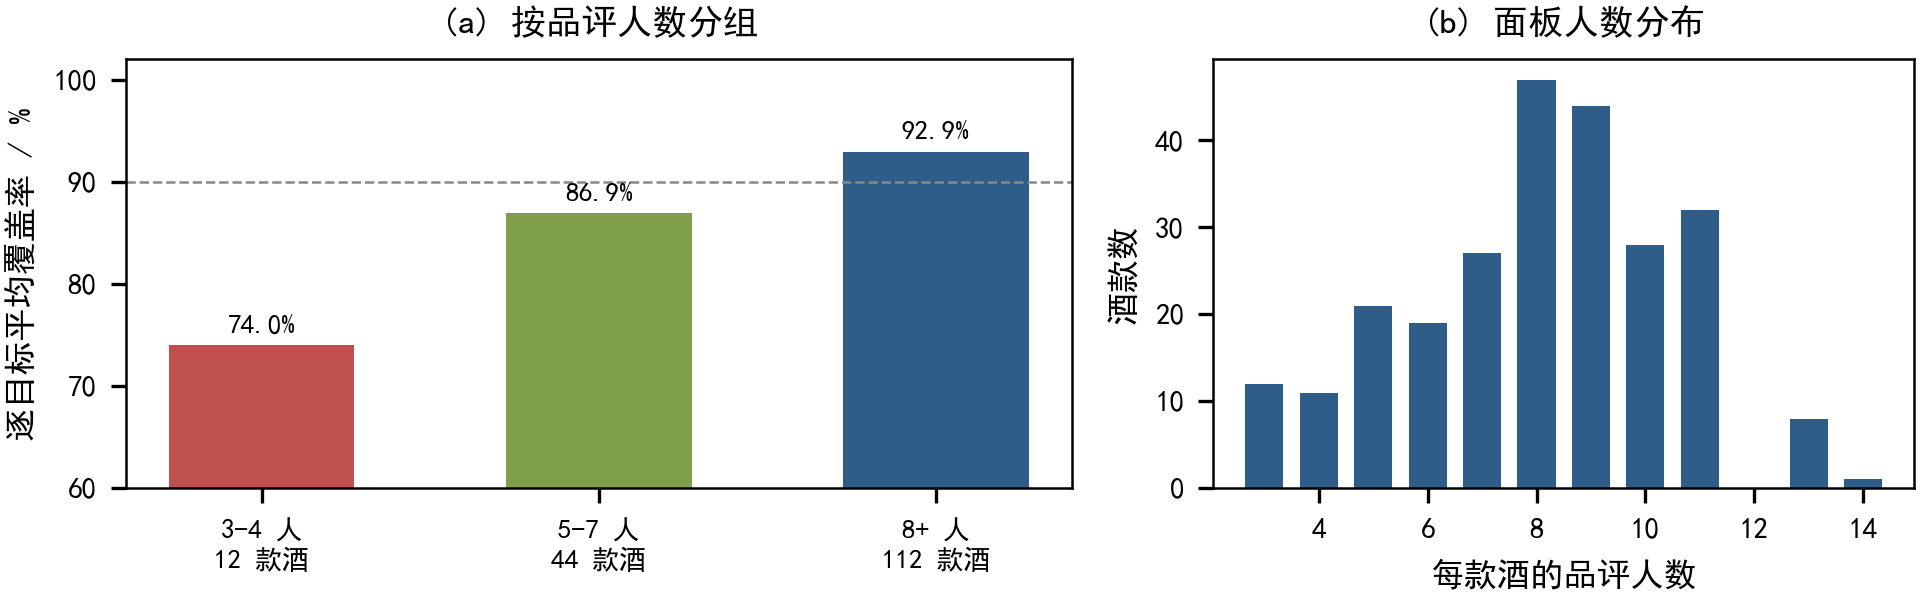
\includegraphics[width=0.95\textwidth]{figures/fig07_coverage.png}
\caption{按品评人数分组的保形区间覆盖率与面板人数分布。覆盖率随人数增加而上升，3—4 人组仅 74.00\%，边际覆盖不能保证小面板目标的条件覆盖。}
\label{fig:cov}
\end{figure*}

\begin{figure}[t]
\centering
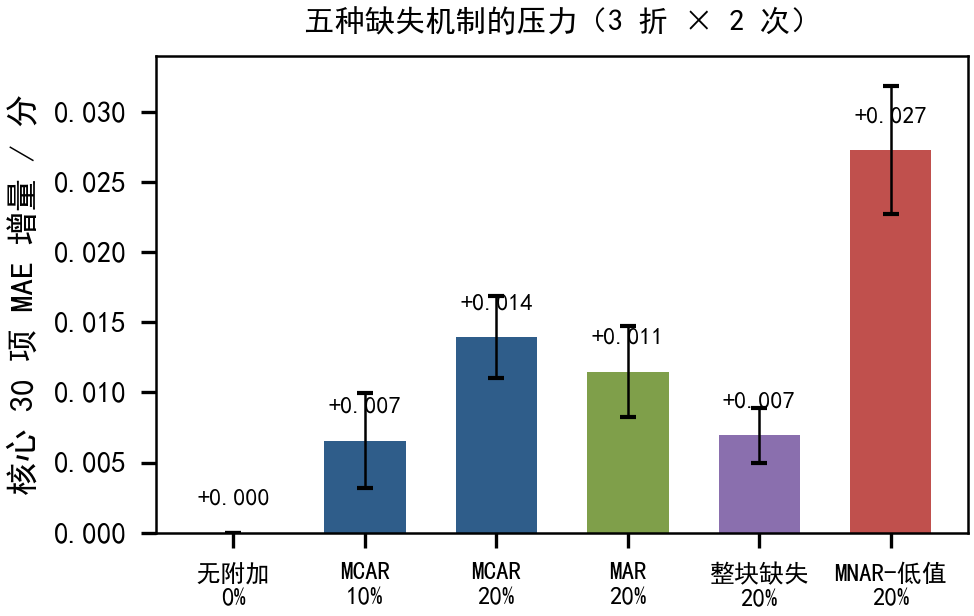
\includegraphics[width=0.95\columnwidth]{figures/fig08_missing_exp.png}
\caption{五种缺失条件下的核心 30 项 MAE 增量（基准 ET-300，0.50666）。系统性低值缺失的代价约为随机缺失的两倍；同为 20\% 时，整块通道缺失的代价最小。}
\label{fig:missexp}
\end{figure}

\subsection{讨论：风格信息与化学输入}

风格中位数基线在核心30项上达到0.50969分，融合模型为0.50222分，两者的固定留出预测重采样区间包含零。两者使用的信息不同：风格基线需要已知风格，融合模型使用化学字段；它们之间的误差差异不能分解为各类信息的独立贡献。

在同样获得风格标签的ET对照中，加入化学字段使核心MAE从0.51701降至0.50275，相对仅风格ET的固定预测重采样区间未跨零。这一结果表明化学字段在该模型和划分下提供了可用的预测信息；然而与风格中位数比较的区间跨零，不能概括成对所有风格基线都有稳定提升。新对照属于审查后的探索性实验，需用新酒样或预先确定的后续划分检验。

等级预测仍有明显短板。核心属性观测众数为0的比例为78.03\%，频率ET的总体一致率为80.52\%，非零众数一致率为24.33\%。宏平均F1、平衡准确率和等级MAE展示不同的模型排序，因而部署时应根据错判非零等级与等级距离的代价选择决策指标。逐属性和逐风格结果用于确定哪些目标需要补充数据或专门建模。

第二问的Top-3基于标准化岭回归系数筛选，并结合重采样与置换贡献分层；这些条件关联和相关网络不能直接解释为因果作用。第三问的生成画像沿用预测端点，其候选还需经过缺陷约束、独立训练代理与实际制备验证。
